% Modelo baseado no hepthesis para monografias, dissertações e teses
% Alan Robert Resende de Freitas

%% Para compilar rascunhos normais (figuras não mostradas para compilação mais rápida)
%\documentclass[hyperpdf,nobind,draft,oneside]{hepthesis}
%\documentclass[hyperpdf,nobind,draft,twoside]{hepthesis}

%% Para compilar rascunhos rápidos (quebra as citações por necessidade)
%\documentclass[hyperpdf,nobind,draft,hidefrontback]{hepthesis}

%% Pacotes que precisam ser incluídos antes do documentclass

%% Para versões de "Cambridge" de capa leve
\documentclass[hyperpdf,bindnopdf]{hepthesis}
%% Para versões de "Cambridge" de capa dura (devem ser de um lado da página apenas)
%\documentclass[hyperpdf,oneside]{hepthesis}

%% Incluia os pacotes no preamble.tex por questão de conveniência
\usepackage[utf8]{inputenc}
\usepackage[english]{babel}

\usepackage{lmodern}

\usepackage{graphicx}
\graphicspath{{R/}}
\usepackage{tikz}

\usepackage{verbatim}

\usepackage[style=authoryear,sorting=ynt]{biblatex}
\addbibresource{masters_dissertation.bib}


\title{My master}
\author{Raniere Gaia Costa da Silva}

\makeatletter
\@ifpackageloaded{hyperref}{%
\hypersetup{%
  pdftitle = {My master},
  pdfsubject = {Raniere Gaia Costa da Silva},
  pdfkeywords = {Image},
  pdfauthor = {\textcopyright\ Raniere Gaia Costa da Silva}
}}{}
\makeatother

%% Começa aqui o documento
\begin{document}

%% Começa aqui o front matter não numerado (páginas de frentes, rubricas e índice)
\begin{frontmatter}
  %!TEX root = ./main.tex

%% Title
\titlepage[Universidade Federal de Ouro Preto]{%
  Tese submetida ao Programa de Pós-Graduação em Ciência da Computação da Universidade Federal de Ouro Preto para obtenção do título de doutor em Ciência da Computação}

%% Resumo
\begin{abstract}[\thetitle \\ \vspace*{1cm} Resumo]
  %\thispagestyle{empty}
Como um dos maiores problemas é que... 
Este é um problema não resolvido pois...
Este trabalho `` \thetitle '' descreve ... 
Os resultados são que ...
\end{abstract}

\begin{abstract}[Title in English \\ \vspace*{1cm} Abstract]
  %\thispagestyle{empty}
One problem with $X$ is that... 
This is an unsolved problem because...
This work describes... 
Our results show that...
\end{abstract}


%% Declaração
\begin{abstract}[Declaração]
Esta tese é resultado de meu próprio trabalho, exceto onde referência explícita é feita ao trabalho de outros, e não foi submetida para obtenção de título nesta nem em outra universidade.
  \vspace*{1cm}
  \begin{flushright}
    Alan Robert Resende de Freitas
  \end{flushright}
\end{abstract}


%% Agradecimentos
\begin{abstract}[Agradecimentos]
Agradeço a \emph{meus pais}, por \dots.

Agradeço a \emph{minha família}, por \dots.

Agradeço a \dots.

Agradeço a \dots.

Agradeço a \dots.

Agradeço a \dots.

Agradeço a \dots.
\end{abstract}


%% Prefácio
\begin{abstract}[Prefácio]
%Resumo expandido... O prefácio é opcional. Aqui você pode explicar a que tipo de leitor se digire o texto.
\end{abstract}

%% ToC
\tableofcontents
% Lista de figuras
\listoffigures
% Insere lista de tabelas
\listoftables
% Insere lista de algoritmos (este comando está disponível se você utilizar o pacote algorithm2e)
% \listofalgorithms

%% Aqui você pode colocar uma citação antes de começar a introdução
% Esta citação é estritamente opcional
\frontquote{%
  Ser ou não ser.}%
  {William Shakespeare, 1564 -- 1616}
%% I don't want a page number on the following blank page either.
\thispagestyle{empty}

\end{frontmatter}

%% Aqui começa o conteúdo mesmo da dissertação
\begin{mainmatter}

  \chapter{Introduction}

%% Reinicie a numeração para garantir que esta seja definitivamente a página #1!
\pagenumbering{arabic}

CRIC \cite{mariarputham2015nominated}

We provide examples using \cite{scikit-image}


  \chapter{Support Vector Machine}

Support vector machines (SVMs)
are a set of supervised learning methods used for classification.
As a supervised learning method,
we expected that
by providing training samples
and fitting the model,
we will receive predictions for new values.

\input{R/svm-intro}


%%% Local Variables:
%%% mode: latex
%%% TeX-master: "masters_dissertation"
%%% End:

  
  \chapter{Digital Image Processing}

We worked with images from
CRIC Database.
% TODO Add citation
The 400 images
have \(1376~\times~1020\)~pixels.

\begin{figure}
  \centering
  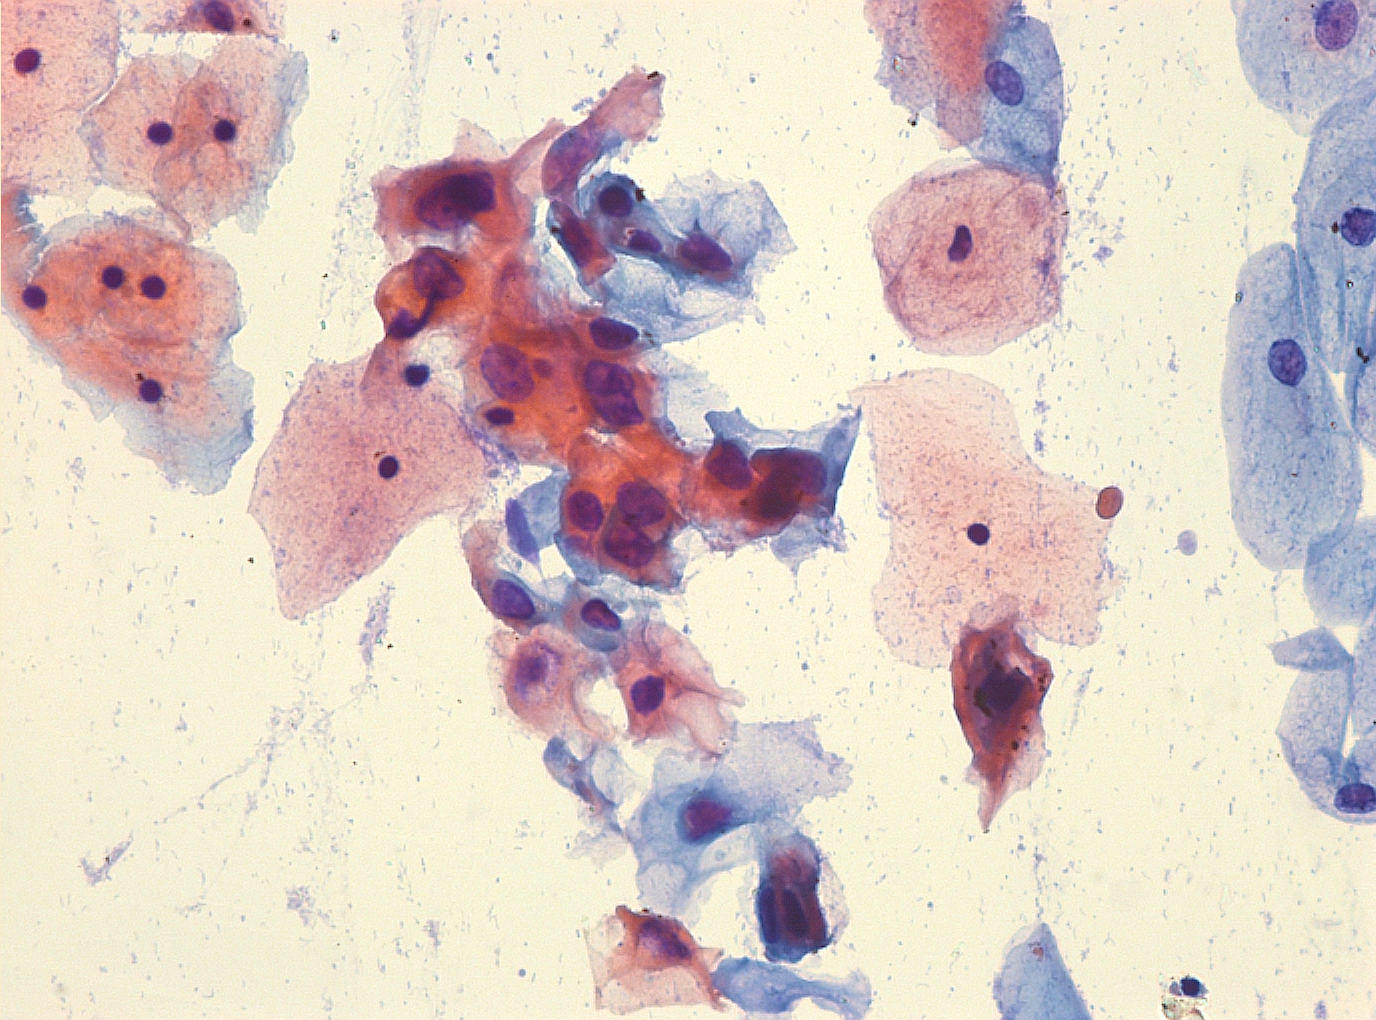
\includegraphics{R/img/be340ee72689dfe3f8dc9c24de6127f4.png}
  \caption{Example of image from CRIC}
  % TODO Add DOI
\end{figure}

We store the image as 3-D array \(A\),
containing
\(M\) rows,
\(N\) columns,
and
3 channels
(red, green, and blue).
For clarity
and
convenience,
since we used Python as programming language,
we use integer values for the discrete coordinates:
\(x = 0, 1, 2, \ldots, M - 1\),
\(y = 0, 1, 2, \ldots, N - 1\),
\(z = 0, 1, 2\).
\(x\), \(y\), and \(z\)
are referred as spatial variables.

The value \(a_{x, y, z}\)
is referred as intensity of \(A\)
at \(x\), \(y\), and \(z\)
and they are integers
in the interval
\([0, 255]\).

A pixel \(p\)
at coordinates \((x, y, z\)
has four horizontal and vertical neighbours,
denoted by \(N_4(p)\):
\begin{itemize}
\item \(x - 1, y, z\)
\item \(x + 1, y, z\)
\item \(x, y - 1, z\)
\item \(x, y + 1, z\)
\end{itemize}
It also has for diagonal neighbours,
denoted by \(N_D(p)\):
\begin{itemize}
\item \(x - 1, y - 1, z\)
\item \(x + 1, y - 1, z\)
\item \(x + 1, y + 1, z\)
\item \(x - 1, y + 1, z\)
\end{itemize}
The \(N_4(p) \cup N_D(p)\)
is called 8-neighbours of \(p\)
and denoted by \(N_8(p)\).

%%% Local Variables:
%%% mode: latex
%%% TeX-master: "masters_dissertation"
%%% End:

  
  \chapter{Texture}

\input{R/range.tex}

\input{R/variance.tex}

  
\end{mainmatter}

%% Aqui você criar novos capítulos e colocar nos apêndices no seu texto
% No apêndice colocamos dados que comprovam nossa pesquisa mas que não são fundamentais para o entendimento do texto
\begin{appendices}
  %% A chamada a "\appendix" já foi feita na declaração do ambiente "appendices"
\chapter{Apêndice}

\section{Dados utilizados para os testes}

Aqui trazemos alguns dados utilizados nos testes que não são fundamentais para entender o texto.

\section{Configurações Especiais}

Aqui temos uns resultados de configurações \dots.

% Se o apêndice for muito grande, ele pode ser separado em vários arquivos, como os arquivos com os capítulos
\end{appendices}

%% Aqui inserimos a contra capa do nosso texto
% A contra capa contém a bibliografia no formato ABNT e um Índice Remissivo
\begin{backmatter}
  \printbibliography

%% Várias pessoas preferem colocar estas tabelas aqui em vez de deixar a front matter enorme. 
%\listoffigures
%\listoftables

%% Aqui você pode incluir um índice remissivo. O índice remissivo organiza os termos importantes do seu texto por ordem alfabética. Para que um termo apareça no índice remissivo, ele precisa estar marcado com o comando \index no seu texto. Isso pode ser feito após a declaração das seções. O MakeIndex deve ser rodado no seu main.tex para gerar este indice.
%\printindex

\end{backmatter}

%% Fecha o documento
\end{document}
